%!TEX root = ../sbc-template.tex

As \emph{Smart} TVs são tidas como aparelhos de televisão com capacidades interativas ligadas à internet, como aplicativos disponíveis em lojas; acesso a conteúdo online como notícias, previsão do tempo, informações de mercados de ações, mapas e jogos; \emph{e-commerce}; navegação web e acesso a redes sociais. Estes aparelhos podem ser equipadas com câmeras e microfones embutidos, além de óculos 3D, como mostra a Figura \ref{fig:smart_samsung}. Estas televisões utilizam os mesmos sistemas operacionais e conjuntos de aplicativos que computadores comuns, o que as torna sucetíveis às mesmas falhas e ataques de segurança que outros dispositivos semelhates. Contudo, \emph{Smart} TVs que adotem o padrão de compartilhameto de mídia DLNA(Digital Living Network Alliance) podem exibir conteúdos como filmes, imagens, músicas e outros diretamente de outros dispositivos como computadores e smartphones que estejam conectados à mesma rede sem fio \cite{michele2014watch}, \cite{shin2013smart}, \cite{perakakis2015proposed}, \cite{whatisasmarttv}.
\begin{figure}
	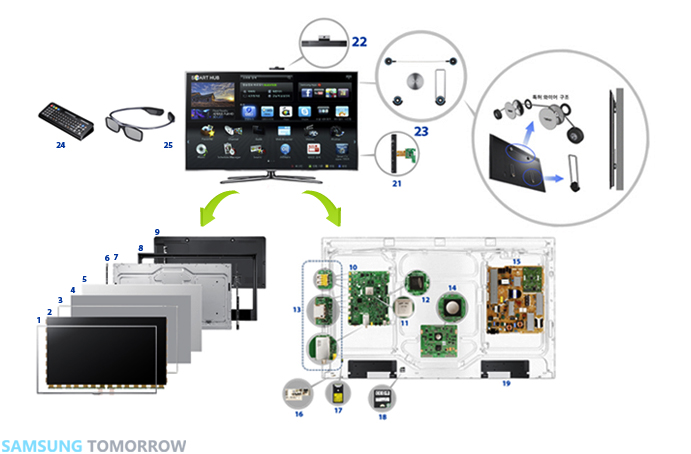
\includegraphics[width=\textwidth]{img/smart_samsung.jpg}
	\caption{\emph{Smart} TV Samsung \cite{samsung:smarttv}}
	\label{fig:smart_samsung}
\end{figure}

A Figura \ref{fig:smart_samsung} exibe um diagrama representativo de uma \emph{Smart} TV. As legendas para os números apresentados na imagem estão na Tabela \ref{tab:smart}.

\begin{table}{h!}
	\centering
	\caption{Legenda da Figura \ref{fig:smart_samsung}}
	\label{tab:smart}
	\begin{tabular}{c l}
		\hline
		Número & Descrição \\
		\hline
		1 & Moldura \\
		2 & Painel de cristal negro (celula) \\
		3 & Molde da moldura do meio \\
		4 & Folha óptica \\
		5 & LGP (Light Guide Plate) -- Prato guia leve \\
		6 & LED \\
		7 & Chassi traseiro \\
		8 & Cobertura do meio \\
		9 & Cobertura traseira \\
		10 & Placa de circuito principal (Placa mãe) \\
		11 & Smart Real Engine \\
		12 & Speed Backlite Engine \\
		13 & Sintonizador, 4 portas HDMI e 3 portas USB \\
		14 & 3D Hyper Real Engine \\
		15 & Placa de Alimentação \\
		16 & Sensor de luz ambiente \\
		17 & Módulo bluetooth \\
		18 & Módulo WiFi \\
		19 & Auto-falantes \\
		20 & Suporte quadrangular \\
		21 & Botão touch operacional \\
		22 & Câmera de video de telefone \\
		23 & Suporte de parede \\
		24 & Controle remoto QWERTY \\
		25 & Óculos 3D \\
		\hline
	\end{tabular}
\end{table}
